\documentclass[11pt,a4paper]{article}

\usepackage[margin=22mm]{geometry}
\usepackage{amsmath,amssymb,booktabs}
\usepackage{tikz,pgfplots}
\usepackage{xcolor,hyperref,siunitx}
\usetikzlibrary{arrows.meta,positioning,calc,decorations.pathreplacing,shapes.geometric}
\pgfplotsset{compat=1.18}
\hypersetup{colorlinks=true,linkcolor=blue,urlcolor=blue}
\sisetup{round-mode=places,round-precision=3}

\definecolor{space}{HTML}{102A43}
\definecolor{orbit}{HTML}{0077B6}
\definecolor{burn}{HTML}{D00000}
\definecolor{fuel}{HTML}{2A9D8F}
\definecolor{panel}{HTML}{EAF4F4}

\title{Physics and Control Architecture\\\large AI-Optimized Nanosatellite Constellation Manager}
\author{Technical Companion to the Python Simulation}
\date{\today}

\begin{document}
\maketitle
\tableofcontents
\newpage

\section{Purpose and scope}
This document explains the physics represented by the project and how its code maps to an engineering workflow. The current implementation has two deliberately separate layers:

\begin{enumerate}
  \item \textbf{Authoritative trajectory layer.} A Two-Line Element set (TLE) is propagated using SGP4. Its output is an inertial position and velocity in the True Equator Mean Equinox (TEME) frame, transformed to the Earth-fixed ITRS/ECEF frame for ground tracks.
  \item \textbf{Control and resource layer.} A transparent, simplified mean-altitude model applies virtual orbital decay, commands an altitude-restoration burn, and tracks propellant through the rocket equation.
\end{enumerate}

The control layer intentionally does \emph{not} edit a TLE or claim to re-propagate an SGP4 orbit after a burn. This keeps the dashboard honest: the map is TLE/SGP4-derived, while the resource telemetry is a station-keeping demonstration model. A maneuver-aware numerical propagator is the appropriate later upgrade.

\section{End-to-end data flow}
\begin{figure}[h]
\centering
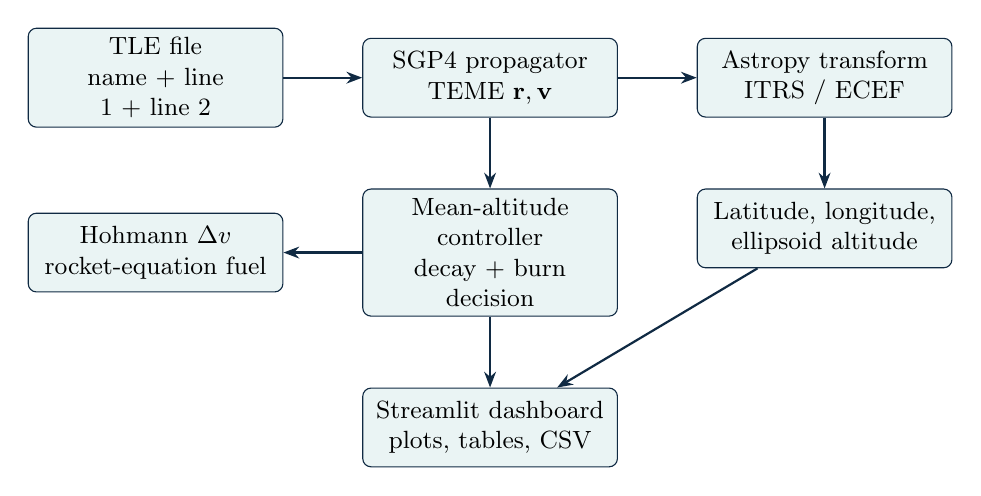
\begin{tikzpicture}[node distance=9mm and 10mm, every node/.style={font=\small}, box/.style={draw=space, rounded corners=3pt, fill=panel, minimum height=10mm, align=center, text width=30mm}, arrow/.style={-{Stealth[length=2mm]}, thick, draw=space}]
\node[box] (tle) {TLE file\\name + line 1 + line 2};
\node[box, right=of tle] (sgp) {SGP4 propagator\\TEME $\mathbf r,\mathbf v$};
\node[box, right=of sgp] (frames) {Astropy transform\\ITRS / ECEF};
\node[box, below=of frames] (geo) {Latitude, longitude,\\ellipsoid altitude};
\node[box, below=of sgp] (control) {Mean-altitude controller\\decay + burn decision};
\node[box, left=of control] (rocket) {Hohmann $\Delta v$\\rocket-equation fuel};
\node[box, below=of control] (dash) {Streamlit dashboard\\plots, tables, CSV};
\draw[arrow] (tle) -- (sgp);
\draw[arrow] (sgp) -- (frames);
\draw[arrow] (frames) -- (geo);
\draw[arrow] (sgp) -- (control);
\draw[arrow] (control) -- (rocket);
\draw[arrow] (control) -- (dash);
\draw[arrow] (geo) -- (dash);
\end{tikzpicture}
\caption{The trajectory and control models share time and satellite identity, but are intentionally distinguishable.}
\end{figure}

\section{Orbital state from a TLE}
\subsection{SGP4 propagation}
A TLE encodes mean orbital elements at a reference epoch. SGP4 uses those elements, Earth-gravity constants, and standard perturbation terms to calculate an Earth-orbiting object's state at a requested UTC epoch:
\begin{equation}
  \left(\mathbf r_{\mathrm{TEME}}(t),\mathbf v_{\mathrm{TEME}}(t)\right)=\operatorname{SGP4}(\mathrm{TLE},t).
\end{equation}
The output units used by the Python \texttt{sgp4} package are kilometres and kilometres per second. SGP4 is particularly suitable for TLE-defined LEO tracking because the TLE itself is fitted to the SGP4 model.

\subsection{From TEME to Earth-fixed coordinates}
TEME is quasi-inertial, whereas a ground map must rotate with Earth. The program uses Astropy's time-aware coordinate transformation to form an ITRS/ECEF vector:
\begin{equation}
  \mathbf r_{\mathrm{ECEF}}(t)=\mathbf R_{\mathrm{TEME}\rightarrow\mathrm{ITRS}}(t)\,\mathbf r_{\mathrm{TEME}}(t).
\end{equation}
The transformation depends on Earth orientation and time, not simply a fixed $z$-axis rotation. The ECEF vector is converted to geodetic latitude $\phi$, longitude $\lambda$, and ellipsoidal height $h$ using WGS-84.

\begin{figure}[h]
\centering
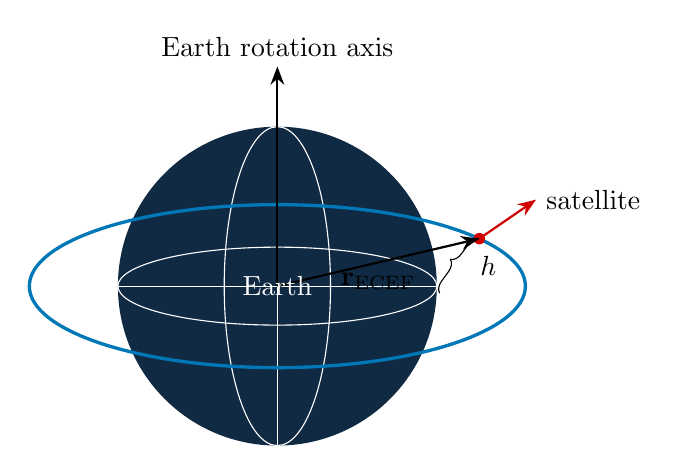
\begin{tikzpicture}[scale=0.9, >=Stealth]
\fill[space] (0,0) circle (2.25);
\draw[white, thin] (0,0) ellipse (2.25 and .55);
\draw[white, thin] (0,0) ellipse (.75 and 2.25);
\draw[white, thin] (-2.25,0) -- (2.25,0);
\draw[white, thin] (0,-2.25) -- (0,2.25);
\draw[orbit, very thick] (0,0) ellipse (3.5 and 1.15);
\fill[burn] (2.85,.67) circle (2.3pt);
\draw[burn, -{Stealth}, thick] (2.85,.67) -- (3.65,1.22) node[right, black] {satellite};
\draw[-{Stealth}, thick] (0,0) -- (2.85,.67) node[midway, below] {$\mathbf r_{\mathrm{ECEF}}$};
\draw[-{Stealth}, thick] (0,0) -- (0,3.1) node[above] {Earth rotation axis};
\draw[decorate,decoration={brace,amplitude=4pt}] (2.29,-.1) -- (2.85,.67) node[midway,right=4pt] {$h$};
\node[white] at (0,0) {Earth};
\end{tikzpicture}
\caption{Earth-fixed geometry used by the ground-track view. The actual software computes the frame conversion rather than using this drawing's simplified geometry.}
\end{figure}

\section{Mean orbit altitude used by the controller}
Instantaneous geodetic altitude rises and falls around an eccentric orbit; it is therefore a poor direct trigger for station keeping. Instead, the controller derives an approximate mean orbit altitude from TLE mean motion $n$:
\begin{align}
 n_{\mathrm{rad/s}} &= \frac{n_{\mathrm{rad/min}}}{60}, \\
 a &= \left(\frac{\mu_\oplus}{n_{\mathrm{rad/s}}^2}\right)^{1/3}, \\
 h_{\mathrm{mean}} &= a-R_\oplus,
\end{align}
where $\mu_\oplus=\SI{398600.4418}{km^3\,s^{-2}}$ and $R_\oplus=\SI{6378.137}{km}$. This is a Keplerian mean-orbit estimate used only for the control state.

\section{Station-keeping control loop}
At each simulation step $\Delta t$, the virtual mean altitude loses a prescribed amount:
\begin{equation}
 h_{k+1}^{-}=h_k-\dot h_{\mathrm{decay}}\frac{\Delta t}{\SI{86400}{s}}.
\end{equation}
When $h_{k+1}^{-}$ is below the permitted lower bound $h_{\mathrm{nominal}}-\epsilon$, a maneuver restores it to $h_{\mathrm{nominal}}$. The UI exposes $\dot h_{\mathrm{decay}}$ and $\epsilon$ so that a short simulation can demonstrate a slow real-world process.

\begin{figure}[h]
\centering
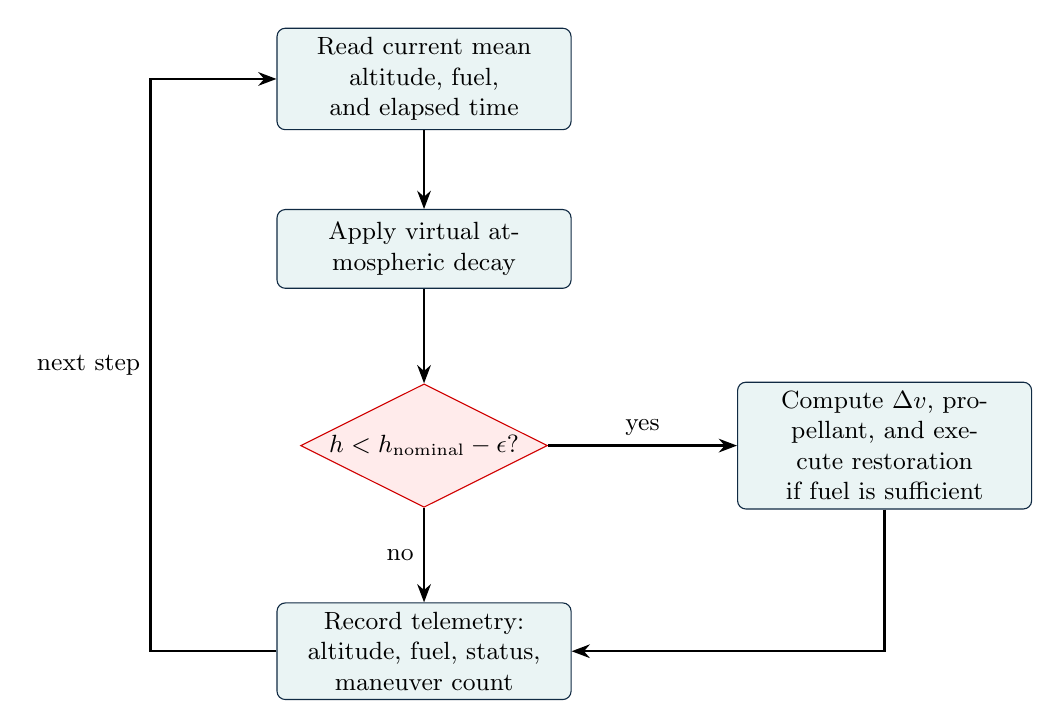
\begin{tikzpicture}[node distance=10mm and 14mm, >=Stealth, every node/.style={font=\small}, proc/.style={draw=space, rounded corners=3pt, fill=panel, align=center, minimum height=10mm, text width=35mm}, decision/.style={diamond, draw=burn, fill=red!8, aspect=2, align=center, inner sep=1pt}, arr/.style={-{Stealth}, thick}]
\node[proc] (start) {Read current mean altitude, fuel, and elapsed time};
\node[proc, below=of start] (decay) {Apply virtual atmospheric decay};
\node[decision, below=of decay, yshift=-2mm] (check) {$h<h_{\rm nominal}-\epsilon$?};
\node[proc, right=of check, xshift=10mm] (burn) {Compute $\Delta v$, propellant, and execute restoration if fuel is sufficient};
\node[proc, below=of check, yshift=-2mm] (record) {Record telemetry:\\altitude, fuel, status, maneuver count};
\draw[arr] (start) -- (decay);
\draw[arr] (decay) -- (check);
\draw[arr] (check) -- node[above] {yes} (burn);
\draw[arr] (check) -- node[left] {no} (record);
\draw[arr] (burn) |- (record);
\draw[arr] (record.west) -| ++(-1.6,0) |- (start.west) node[pos=.25,left] {next step};
\end{tikzpicture}
\caption{Closed-loop deterministic controller. Fuel exhaustion records \texttt{OUT\_OF\_FUEL} rather than pretending a maneuver occurred.}
\end{figure}

\section{Why a small burn raises an orbit}
For a prograde burn, speed rises at the current position. That point becomes the perigee of a new elliptical transfer orbit, whose apogee is higher. A second prograde burn at apogee circularizes the orbit. For a circular-to-circular Hohmann transfer from $r_1$ to $r_2$, the ideal total delta-v is:
\begin{align}
 \Delta v_1 &= \sqrt{\frac{\mu}{r_1}}\left(\sqrt{\frac{2r_2}{r_1+r_2}}-1\right), \\
 \Delta v_2 &= \sqrt{\frac{\mu}{r_2}}\left(1-\sqrt{\frac{2r_1}{r_1+r_2}}\right), \\
 \Delta v_{\mathrm{total}} &= \left|\Delta v_1\right|+\left|\Delta v_2\right|.
\end{align}

\begin{figure}[h]
\centering
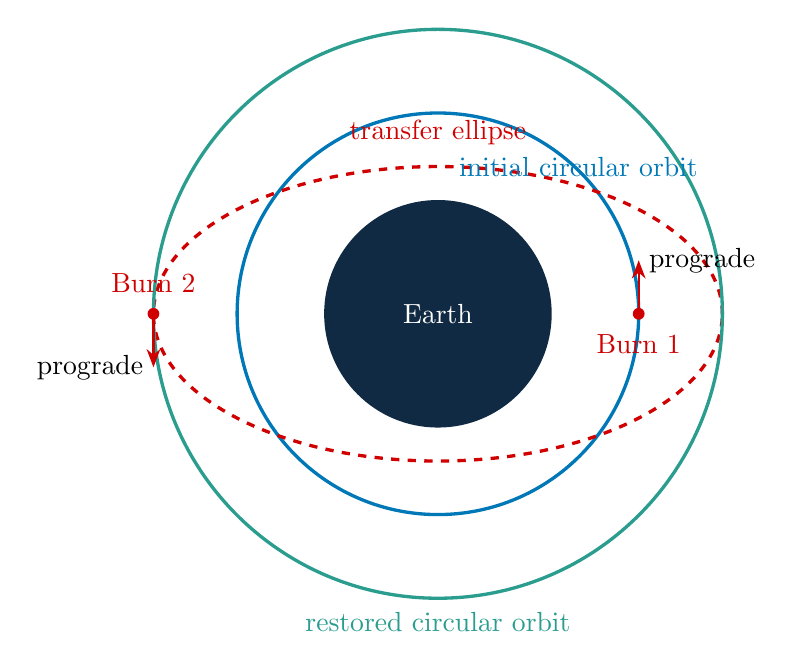
\begin{tikzpicture}[scale=.85, >=Stealth]
\fill[space] (0,0) circle (1.7);
\draw[orbit, very thick] (0,0) circle (3.0);
\draw[burn, very thick, dashed] (0,0) ellipse (4.25 and 2.2);
\draw[fuel, very thick] (0,0) circle (4.25);
\fill[burn] (3,0) circle (2.5pt) node[below=4pt] {Burn 1};
\fill[burn] (-4.25,0) circle (2.5pt) node[above=4pt] {Burn 2};
\draw[-{Stealth}, burn, thick] (3,0) -- (3,0.8) node[right,black] {prograde};
\draw[-{Stealth}, burn, thick] (-4.25,0) -- (-4.25,-.8) node[left,black] {prograde};
\node[orbit] at (2.1,2.2) {initial circular orbit};
\node[burn] at (0,2.7) {transfer ellipse};
\node[fuel] at (0,-4.6) {restored circular orbit};
\node[white] at (0,0) {Earth};
\end{tikzpicture}
\caption{Idealized two-burn orbit raise. The project uses this as an energy-cost estimate, not as a high-fidelity maneuver propagator.}
\end{figure}

\section{Fuel use: the rocket equation}
The Tsiolkovsky rocket equation relates delta-v to a mass ratio:
\begin{equation}
 \Delta v=I_{sp}g_0\ln\left(\frac{m_0}{m_f}\right), \qquad
 m_f=\frac{m_0}{\exp\left(\Delta v/(I_{sp}g_0)\right)}.
\end{equation}
The implementation uses $I_{sp}=\SI{220}{s}$, $g_0=\SI{9.80665}{m\,s^{-2}}$, dry mass $\SI{10}{kg}$, and an initial propellant mass selected in the dashboard. Propellant consumed is $m_0-m_f$. A maneuver is rejected if the computed consumption exceeds fuel remaining.

\section{Illustrative 24-hour controller output}
The following plots are a deterministic illustration using a decay rate of \SI{1}{km/day}, a \SI{0.2}{km} tolerance, and hourly samples. Values are representative of the implemented equations; a run's exact values depend on each satellite's mean altitude.

\begin{figure}[h]
\centering
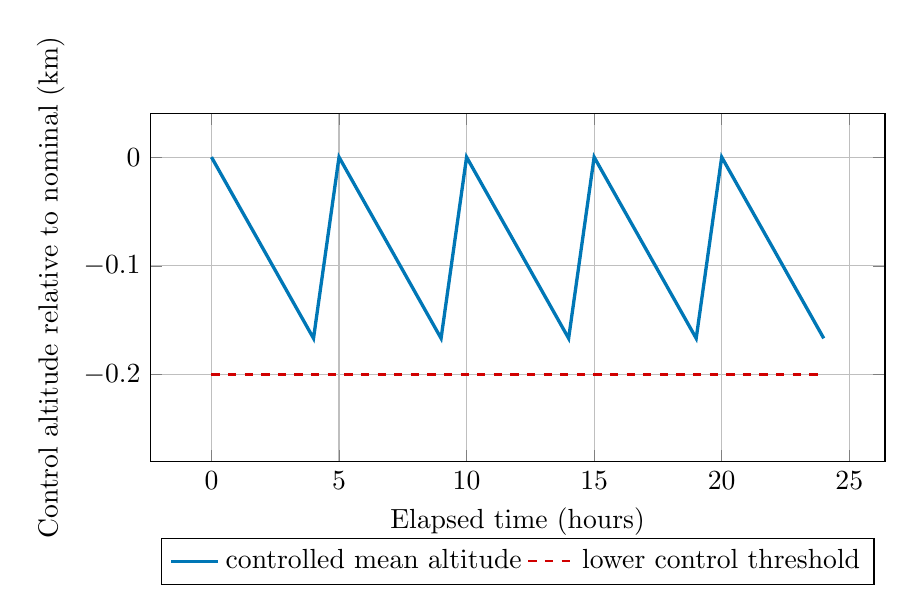
\begin{tikzpicture}
\begin{axis}[width=.9\textwidth,height=6cm,xlabel={Elapsed time (hours)},ylabel={Control altitude relative to nominal (km)},grid=both,legend style={at={(.5,-.22)},anchor=north,legend columns=2},ymin=-.28,ymax=.04]
\addplot[orbit,very thick] coordinates {(0,0)(1,-.0417)(2,-.0833)(3,-.125)(4,-.1667)(5,0)(6,-.0417)(7,-.0833)(8,-.125)(9,-.1667)(10,0)(11,-.0417)(12,-.0833)(13,-.125)(14,-.1667)(15,0)(16,-.0417)(17,-.0833)(18,-.125)(19,-.1667)(20,0)(21,-.0417)(22,-.0833)(23,-.125)(24,-.1667)};
\addlegendentry{controlled mean altitude}
\addplot[burn,dashed,thick] coordinates {(0,-.2)(24,-.2)};
\addlegendentry{lower control threshold}
\end{axis}
\end{tikzpicture}
\caption{Sawtooth behavior of the mean-altitude controller. The next hourly sample would cross the threshold and trigger another restoration.}
\end{figure}

\begin{figure}[h]
\centering
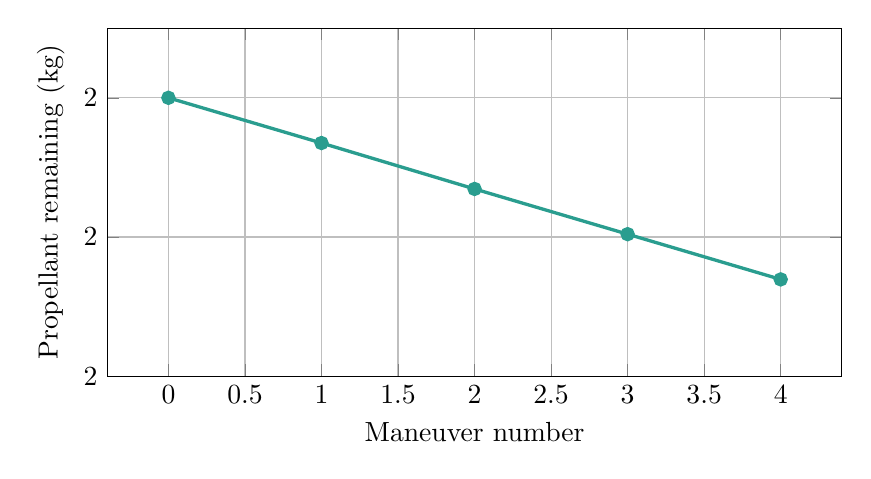
\begin{tikzpicture}
\begin{axis}[width=.9\textwidth,height=6cm,xlabel={Maneuver number},ylabel={Propellant remaining (kg)},grid=both,ymin=1.996,ymax=2.001]
\addplot[fuel,very thick,mark=*] coordinates {(0,2.0000)(1,1.99935)(2,1.99869)(3,1.99804)(4,1.99739)};
\end{axis}
\end{tikzpicture}
\caption{Illustrative propellant depletion for a low-thrust station-keeping sequence. Fuel declines monotonically and never becomes negative.}
\end{figure}

\section{Telemetry dictionary}
\begin{center}
\begin{tabular}{lll}
\toprule
Field & Unit & Meaning \\
\midrule
\texttt{altitude\_km} & km & Instantaneous ellipsoidal altitude from ECEF/ITRS \\
\texttt{mean\_orbit\_altitude\_km} & km & Mean-altitude estimate derived from TLE mean motion \\
\texttt{controlled\_mean\_altitude\_km} & km & Virtual controller state after decay/burn action \\
\texttt{maneuver\_delta\_v\_m\_s} & m/s & Delta-v spent at the current step \\
\texttt{cumulative\_delta\_v\_m\_s} & m/s & Total delta-v spent by that satellite \\
\texttt{fuel\_remaining\_kg} & kg & Remaining virtual propellant \\
\texttt{station\_keeping\_status} & -- & \texttt{NOMINAL}, \texttt{MANEUVER}, or \texttt{OUT\_OF\_FUEL} \\
\bottomrule
\end{tabular}
\end{center}

\section{Model limits and the Phase 3 path}
The present model is appropriate for demonstrating systems engineering connections: TLE ingestion, frame conversion, feedback control, delta-v budgeting, and a dashboard. It is not a mission-design-grade orbit determination system. Specifically, it does not yet include drag density models, covariance propagation, thrust direction errors, eclipse constraints, or post-burn numerical propagation.

Phase 3 should add a rolling conjunction screen: propagate all satellite pairs over a prediction window, calculate closest approach, raise an alert below a keep-out radius, apply a deterministic phasing maneuver, then re-screen. Only after that deterministic baseline is validated should a learned policy be considered.

\end{document}
